\documentclass[tikz,border=10pt]{standalone}
\usepackage{pgfplots}
\usepackage{amsmath}

\begin{document}

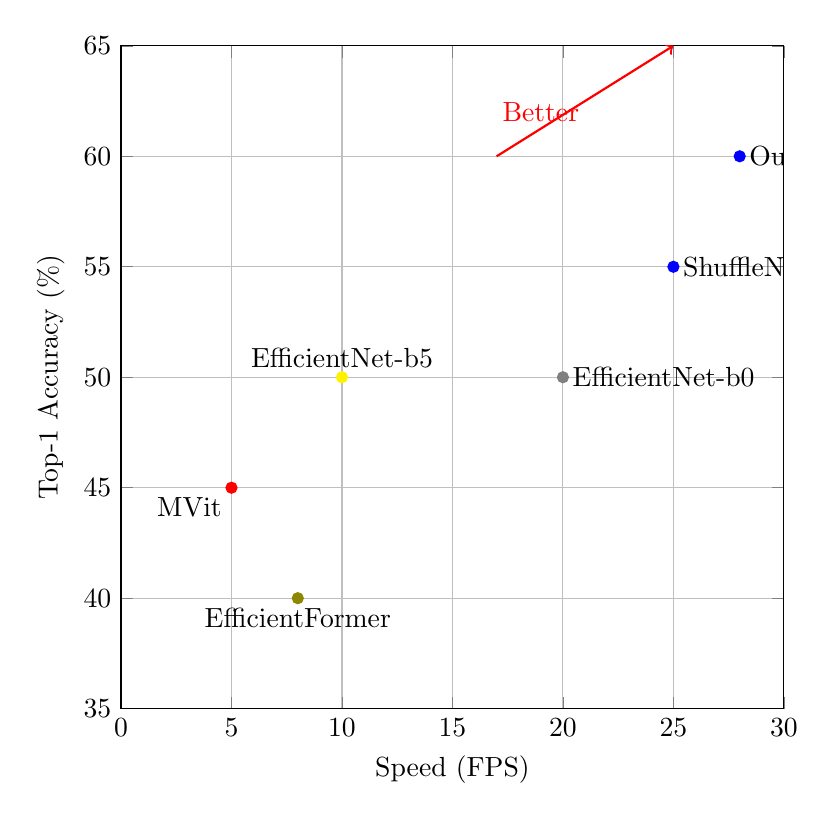
\begin{tikzpicture}
  \begin{axis}[
    width=10cm,
    height=10cm,
    xlabel={Speed (FPS)},
    ylabel={Top-1 Accuracy (\%)},
    xmin=0, xmax=30,
    ymin=35, ymax=65,
    xtick={0,5,10,15,20,25,30},
    ytick={35,40,45,50,55,60,65},
    grid=major,
    scatter/classes={
      a={mark=*,draw=red,fill=red},
      b={mark=*,draw=yellow,fill=yellow},
      c={mark=*,draw=gray,fill=gray},
      d={mark=*,draw=olive,fill=olive},
      e={mark=*,draw=blue,fill=blue}
    }
  ]
  
  \addplot[scatter,only marks,scatter src=explicit symbolic]
  coordinates {
    (5,45) [a] 
    (10,50) [b]
    (20,50) [c]
    (8,40) [d]
    (25,55) [e]
    (28,60) [e]
  };
  
  \node at (axis cs:5,45) [anchor=north east] {MVit};
  \node at (axis cs:10,50) [anchor=south] {EfficientNet-b5};
  \node at (axis cs:20,50) [anchor=west] {EfficientNet-b0};
  \node at (axis cs:8,40) [anchor=north] {EfficientFormer};
  \node at (axis cs:25,55) [anchor=west] {ShuffleNetV2};
  \node at (axis cs:28,60) [anchor=west] {Ours};
  
  \node[red, align=center] at (axis cs:19,62) {Better};
  \draw[->, red, thick] (axis cs:17,60) -- (axis cs:25,65);

  \end{axis}
\end{tikzpicture}

\end{document}